\chapter{Métodos}
\label{metodos}

Este capítulo describe la metodología empleada en el desarrollo del sistema de aprendizaje de idiomas, incluyendo la arquitectura del sistema, la implementación de los componentes, los algoritmos desarrollados y la metodología de evaluación.

\section{Arquitectura del Sistema}
\label{arquitectura-sistema}

El sistema se ha diseñado siguiendo una arquitectura modular y escalable que integra tecnologías de vanguardia en \gls{ia} y procesamiento de lenguaje natural. La arquitectura se divide en dos componentes principales: frontend y backend, comunicados a través de una API REST.

\begin{figure}[H]
	\centering
	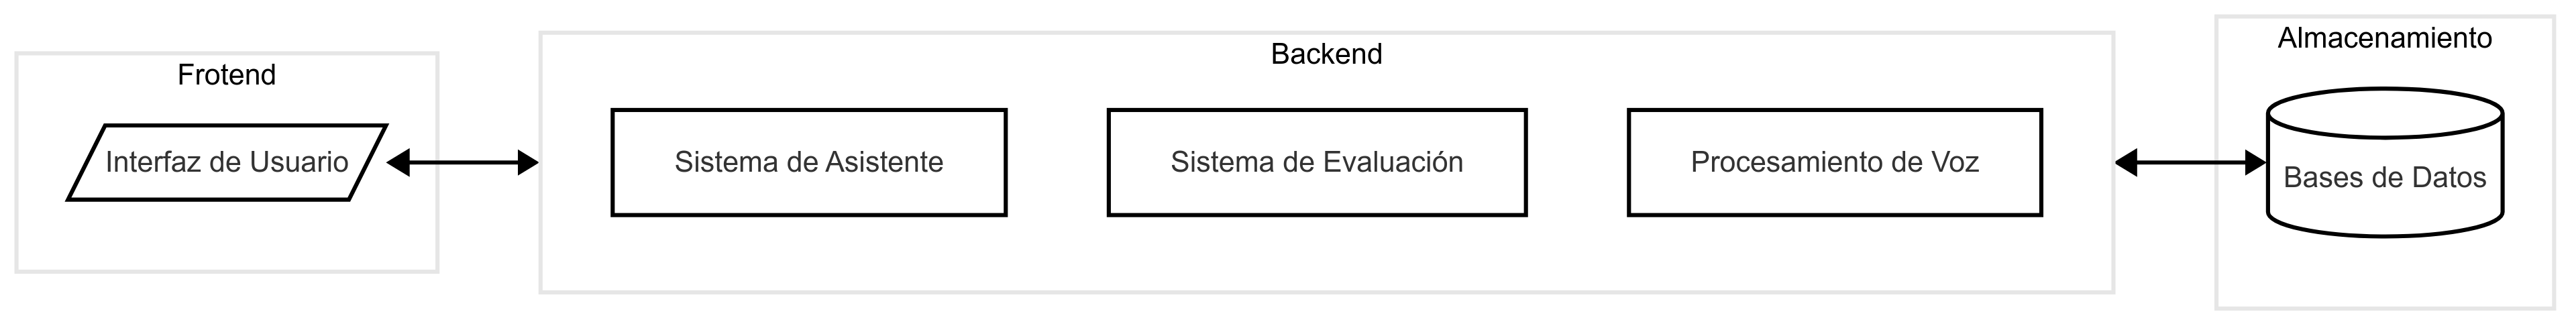
\includegraphics[width=0.8\textwidth]{figuras/system-overview.png}
	\caption{Arquitectura Simplificada del Sistema}
	\label{fig:arquitectura-sistema}
\end{figure}


\subsection{Frontend}
\label{frontend}

El frontend del sistema se implementa utilizando Next.js y está basado en el framework \gls{assistant-ui}, un proyecto \gls{open-source} que facilita la integración de interfaces de chat con LangGraph. Esta decisión arquitectónica permite una rápida implementación de funcionalidades de chat mientras mantiene la flexibilidad para personalizaciones específicas del dominio.

\begin{figure}[H]
	\centering
	\caption{Arquitectura del Frontend}
	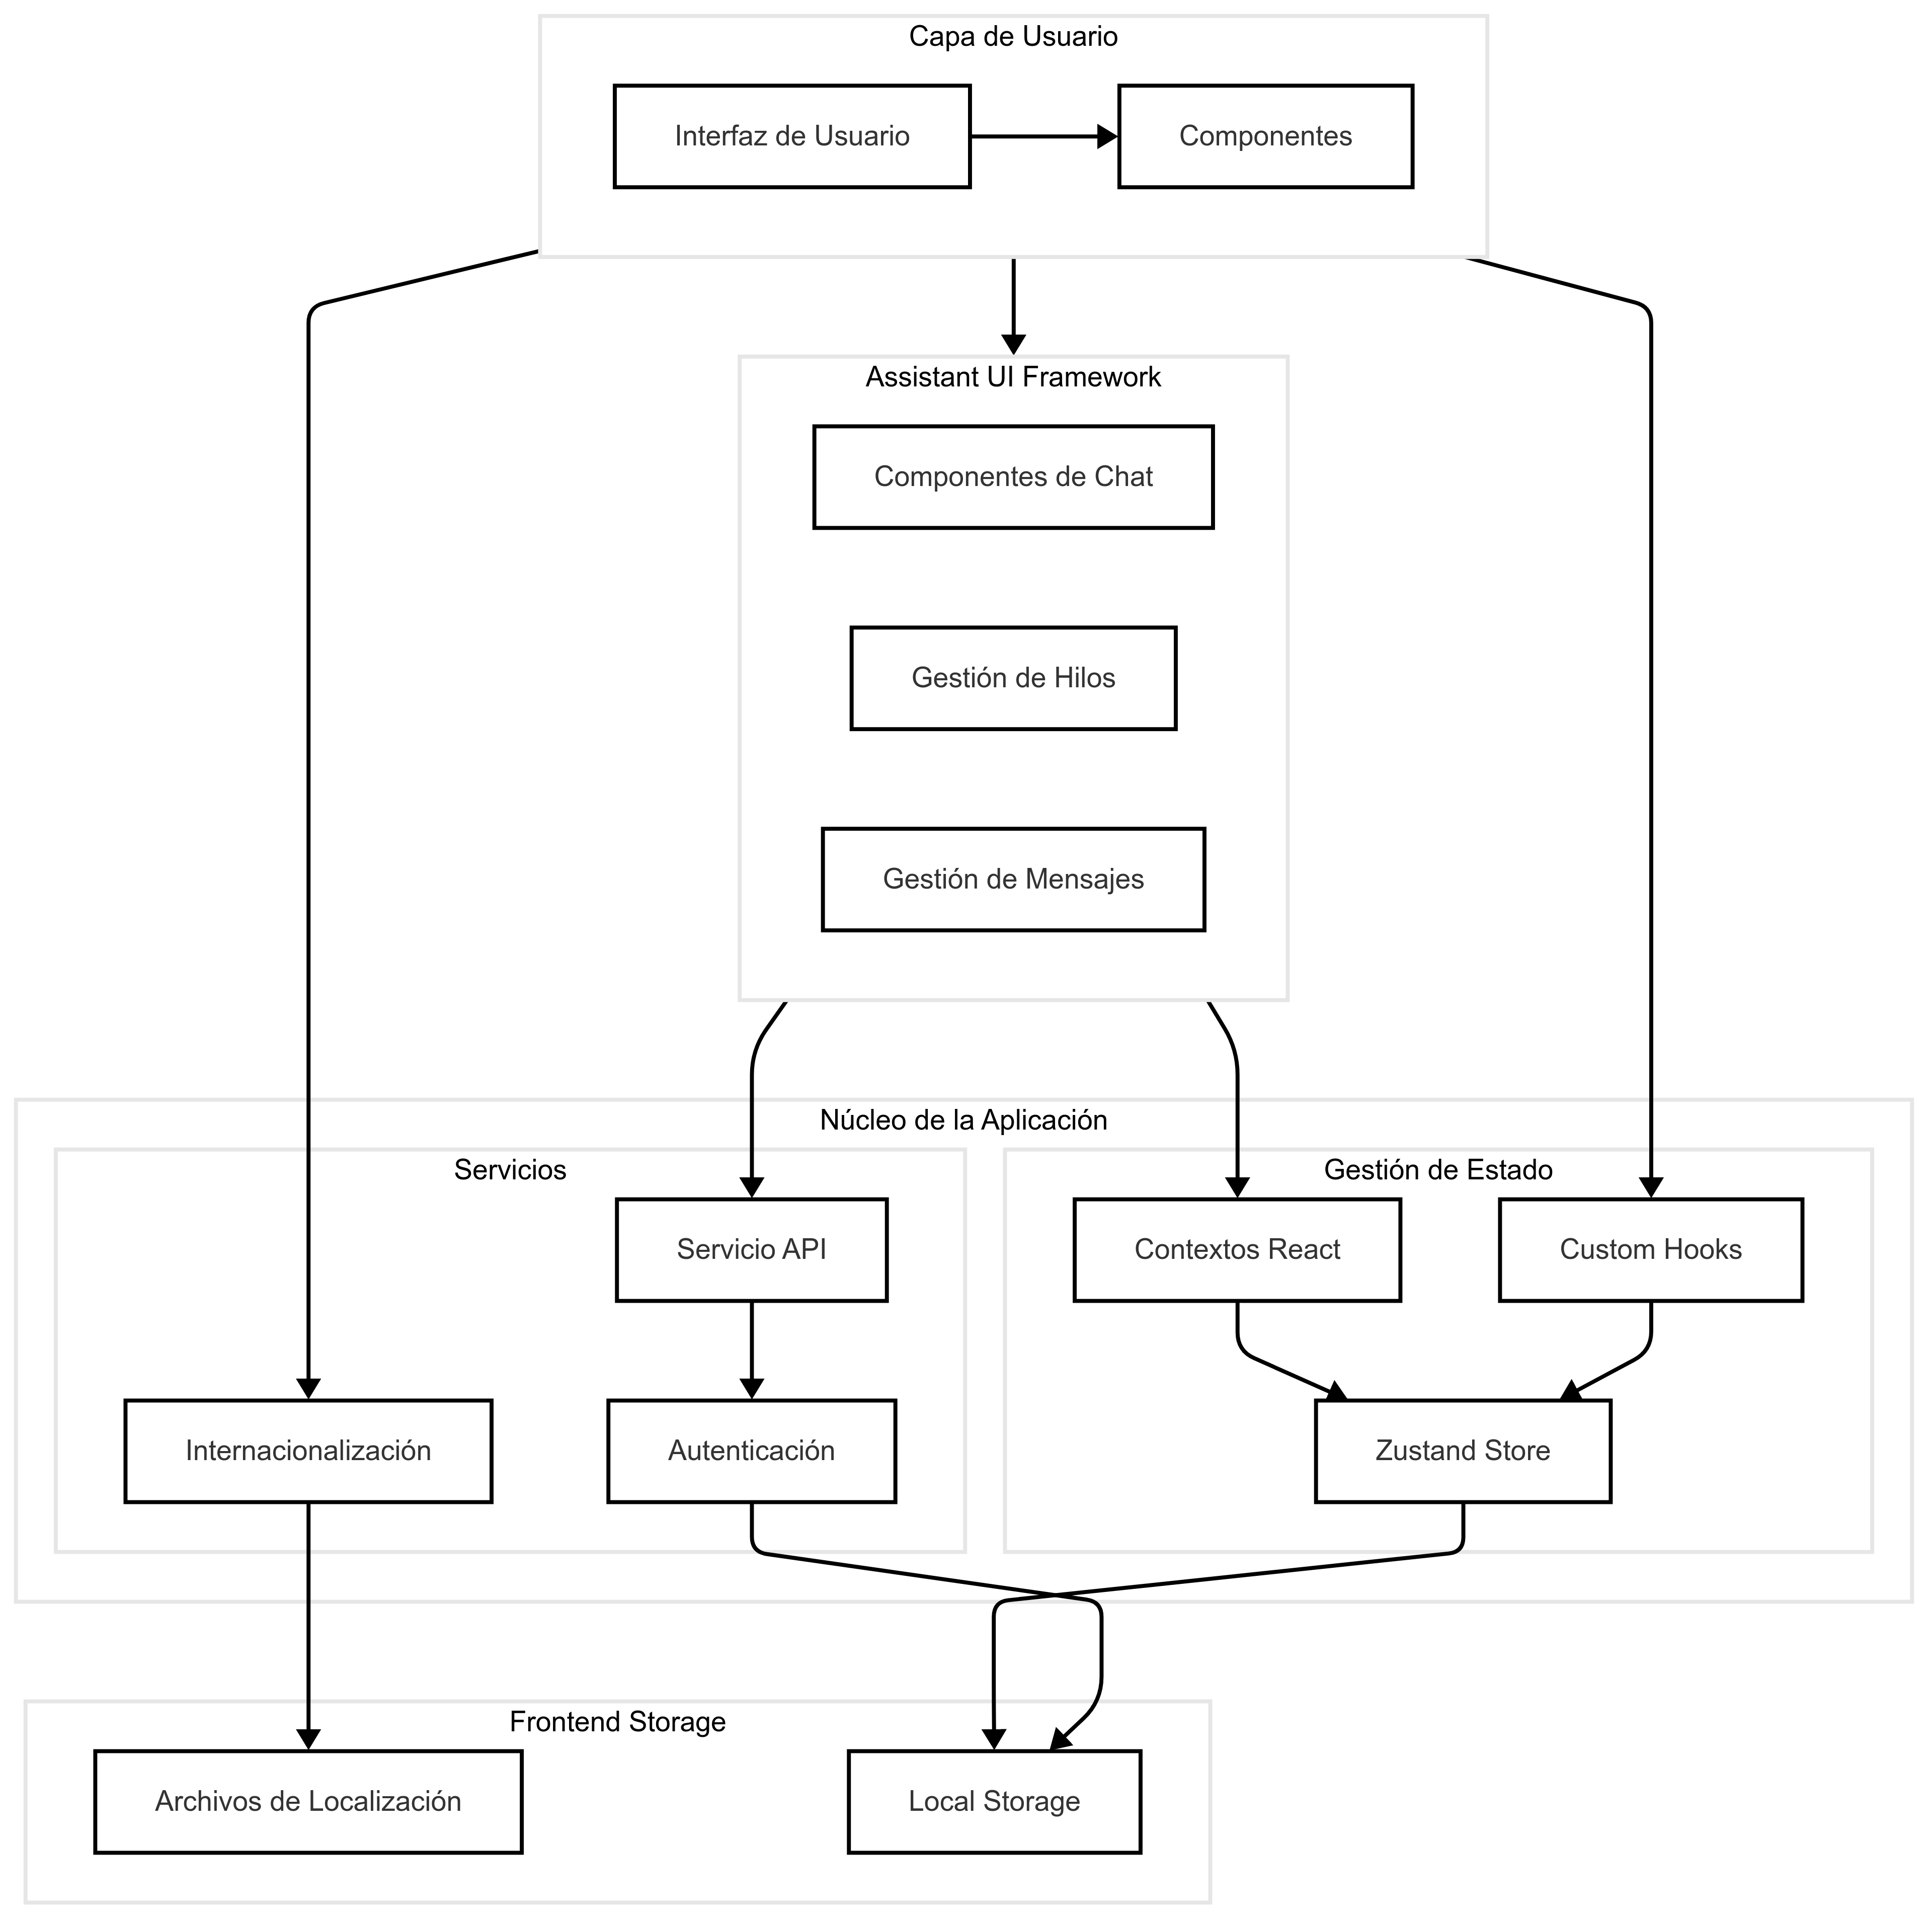
\includegraphics[width=0.8\textwidth]{figuras/frontend.png}
	\label{fig:arquitectura-frontend}
\end{figure}

\subsubsection{Assistant UI Framework}
\label{assistant-ui}

El sistema se construye sobre \gls{assistant-ui}, que proporciona:

\begin{itemize}
	\item \textbf{Componentes de Chat}:
	      \begin{itemize}
		      \item Interfaz de chat prediseñada y personalizable
		      \item Sistema de renderizado de mensajes
		      \item Gestión de entrada de usuario
	      \end{itemize}

	\item \textbf{Gestión de Hilos}:
	      \begin{itemize}
		      \item Sistema de hilos de conversación
		      \item Persistencia de contexto conversacional
		      \item Manejo de múltiples conversaciones
	      \end{itemize}

	\item \textbf{Gestión de Mensajes}:
	      \begin{itemize}
		      \item Sistema de cola de mensajes
		      \item Gestión de estados de mensajes
		      \item Manejo de respuestas asíncronas
	      \end{itemize}
\end{itemize}
\subsubsection{Arquitectura de Componentes}
La arquitectura del frontend se organiza en las siguientes capas:

\begin{itemize}
	\item \textbf{Capa de Usuario}:
	      \begin{itemize}
		      \item Implementación de páginas y rutas utilizando el sistema de enrutamiento de Next.js
		      \item Implementación de layouts y templates adaptables
		      \item Integración con el sistema de internacionalización
	      \end{itemize}

	\item \textbf{Núcleo de la Aplicación}:
	      \begin{itemize}
		      \item Gestión de estado utilizando Zustand para el manejo de datos de roleplay, progreso y reportes
		      \item Servicios para comunicación con el backend
		      \item Sistema de internacionalización con archivos de localización
	      \end{itemize}

	\item \textbf{Utilidades}:
	      \begin{itemize}
		      \item Funciones de validación y formateo
		      \item Manejadores de errores globales
		      \item Helpers para formateo y transformación de datos
		      \item Adaptadores para internacionalización
	      \end{itemize}
\end{itemize}

\subsubsection{Gestión de Estado}
\label{gestion-estado}

El sistema utiliza Zustand como solución de gestión de estado, proporcionando:

\begin{itemize}
	\item \textbf{Estado Global}:
	      \begin{itemize}
		      \item Gestión del estado del roleplay
		      \item Seguimiento del progreso del usuario
		      \item Almacenamiento de reportes de actividad
	      \end{itemize}

	\item \textbf{Persistencia}:
	      \begin{itemize}
		      \item Integración con localStorage para persistencia de datos
		      \item Sincronización de estado entre sesiones
		      \item Gestión de caché de datos
	      \end{itemize}
\end{itemize}

\subsubsection{Servicios de Comunicación}
\label{servicios-comunicacion}

La comunicación con el backend se gestiona a través de servicios especializados:

\begin{itemize}
	\item \textbf{API Service}:
	      \begin{itemize}
		      \item Implementación de cliente HTTP basado en Axios
		      \item Sistema de interceptores para manejo de errores
		      \item Caché de respuestas para optimización de rendimiento
	      \end{itemize}

	\item \textbf{Gestión de Autenticación}:
	      \begin{itemize}
		      \item Sistema de autenticación basado en tokens
		      \item Manejo de sesiones de usuario
		      \item Protección de rutas y recursos
	      \end{itemize}

	\item \textbf{Servicio de Internacionalización}:
	      \begin{itemize}
		      \item Gestión de traducciones y locales
		      \item Cambio dinámico de idioma
		      \item Formateo de fechas y números según la localización
	      \end{itemize}
\end{itemize}

\subsection{Backend}
\label{backend}

El backend del sistema se implementa utilizando FastAPI como framework principal, incorporando un sistema multi-agente basado en LangGraph para la gestión de la lógica de aprendizaje. La arquitectura se organiza en capas claramente definidas que gestionan diferentes aspectos del sistema.

\begin{figure}[H]
	\centering
	\caption{Arquitectura del Backend}
	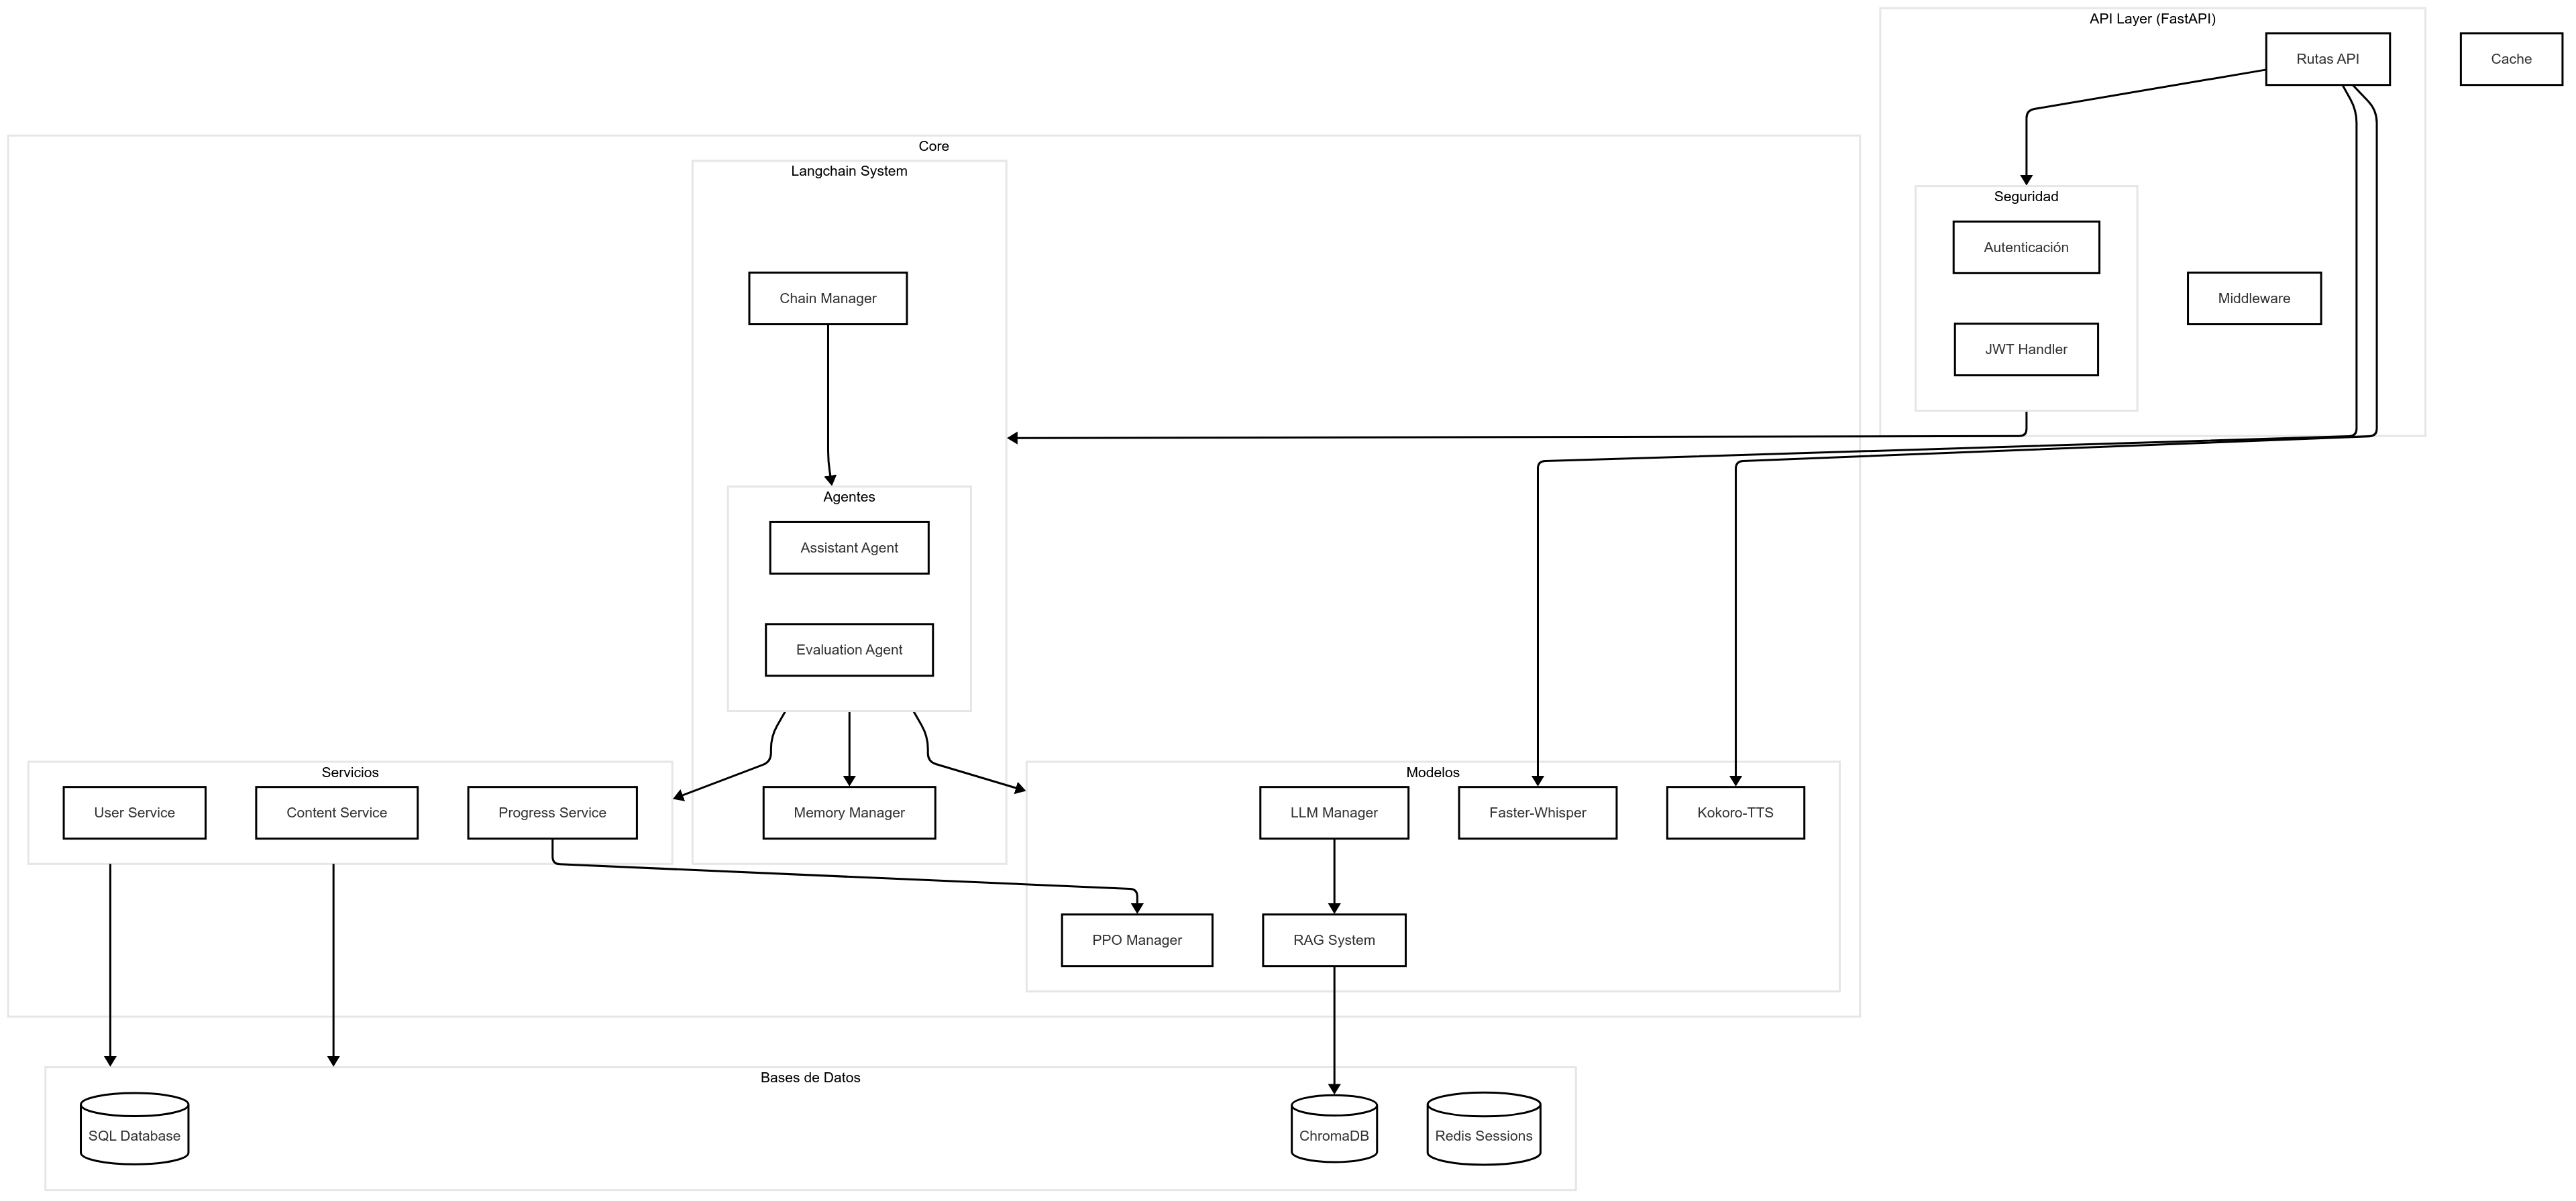
\includegraphics[width=0.8\textwidth]{figuras/backend.png}
	\label{fig:arquitectura-backend}
\end{figure}

\subsubsection{Capa de API}
\label{capa-api}

La capa de API, implementada con FastAPI, gestiona todas las interacciones con el cliente a través de endpoints RESTful. El sistema proporciona:

\begin{itemize}
    \item \textbf{Documentación y Validación}:
    \begin{itemize}
        \item Documentación automática mediante OpenAPI
        \item Validación de datos utilizando Pydantic
    \end{itemize}

    \item \textbf{Seguridad}:
    \begin{itemize}
        \item Autenticación mediante JWT
        \item Rate limiting para prevención de abusos
        \item Sistema de validación de permisos basado en roles
        \item Implementación de CORS para seguridad entre dominios
    \end{itemize}

    \item \textbf{Procesamiento de Voz}:
    \begin{itemize}
        \item Integración con Faster-Whisper para transcripción de voz
        \item Integración con Kokoro-TTS para síntesis de voz
    \end{itemize}
\end{itemize}
\subsubsection{Sistema Multi-Agente}
\label{sistema-multi-agente}

El sistema implementa dos agentes especializados utilizando Langchain:

\begin{itemize}
    \item \textbf{Assistant Agent}: Maneja las conversaciones con el usuario, integrándose con modelos \gls{llm} y utilizando un sistema de \gls{rag} para contextualización.
    
    \item \textbf{Evaluation Agent}: Realiza la evaluación continua del progreso, analiza patrones de error y ajusta los parámetros de aprendizaje utilizando el modelo \gls{ppo}.
\end{itemize}

\subsubsection{Gestión de Modelos}
\label{gestion-modelos}

La integración de modelos de \gls{ia} se realiza a través de gestores especializados:

\begin{itemize}
    \item \textbf{LLM Manager}: Coordina la integración con modelos de lenguaje, gestionando prompts y contextos.
    
    \item \textbf{PPO Manager}: Implementa el algoritmo \gls{ppo}, manejando estados y recompensas para la evaluación.
    
    \item \textbf{RAG System}: Gestiona la indexación de contenido educativo y realiza búsquedas semánticas mediante ChromaDB.
    
    \item \textbf{Modelos de Voz}: Implementa Faster-Whisper para STT y Kokoro-TTS para TTS.
\end{itemize}

\subsubsection{Servicios Core}
\label{servicios-core}

Los servicios principales del sistema incluyen:

\begin{itemize}
    \item \textbf{User Service}: Gestiona perfiles de usuario y preferencias.
    
    \item \textbf{Content Service}: Maneja la gestión y adaptación de recursos educativos.
    
    \item \textbf{Progress Service}: Realiza el seguimiento del avance y se integra con el modelo PPO para la evaluación.
\end{itemize}

\subsubsection{Capa de Datos}
\label{capa-datos}

La gestión de datos se implementa mediante tres sistemas de almacenamiento:

\begin{itemize}
    \item \textbf{SQL Database}: Almacena datos estructurados y relaciones entre entidades.
    
    \item \textbf{ChromaDB}: Base de datos vectorial para embeddings y búsquedas semánticas.
    
    \item \textbf{Redis}: Gestión de sesiones y caché para optimizar el acceso a datos frecuentes.
\end{itemize}

\subsubsection{Optimización y Monitoreo}
\label{optimizacion-monitoreo}

El sistema implementa:

\begin{itemize}
    \item \textbf{Monitoreo}:
    \begin{itemize}
        \item Logging estructurado de eventos
        \item Métricas de rendimiento
        \item Sistema de alertas automáticas
    \end{itemize}

    \item \textbf{Optimización}:
    \begin{itemize}
        \item Caché en múltiples niveles
        \item Pooling de conexiones
        \item Arquitectura stateless
    \end{itemize}
\end{itemize}


\section{Implementación de los Componentes}
\label{implementacion-componentes}

Esta sección detalla la implementación técnica de los componentes principales del sistema: el sistema de agentes y el procesamiento de voz. Cada componente se ha desarrollado considerando los requisitos de rendimiento, escalabilidad y usabilidad del sistema.

\subsection{Sistema de Agentes}
\label{implementacion-agentes}

El sistema implementa dos agentes especializados utilizando Langchain como framework base. Cada agente está diseñado con responsabilidades específicas y utiliza el sistema de memoria de Langchain para mantener el contexto de las interacciones.

\subsubsection{Assistant Agent}

El Assistant Agent se construye sobre un modelo \gls{llm} con un sistema de \gls{rag} para contextualización. Sus principales componentes son:

\begin{itemize}
    \item \textbf{Gestión de Contexto}:
    \begin{itemize}
        \item Mantiene el estado del diálogo mediante el Memory Manager de Langchain
        \item Implementa un sistema de recuperación de contexto relevante
        \item Coordina la integración con el sistema RAG
    \end{itemize}

    \item \textbf{Generación de Respuestas}:
    \begin{itemize}
        \item Utiliza templates dinámicos adaptados al nivel del estudiante
        \item Implementa prompts específicos para diferentes tipos de interacciones
        \item Mantiene la coherencia pedagógica en las conversaciones
    \end{itemize}

    \item \textbf{Integración con Servicios}:
    \begin{itemize}
        \item Coordina con el Content Service para acceso a recursos educativos
        \item Interactúa con el User Service para personalización
        \item Registra interacciones para análisis posterior
    \end{itemize}
\end{itemize}

\subsubsection{Evaluation Agent}

El Evaluation Agent implementa un sistema de evaluación continua que utiliza el modelo \gls{ppo} para optimizar las evaluaciones. Sus componentes principales incluyen:

\begin{itemize}
    \item \textbf{Sistema de Evaluación}:
    \begin{itemize}
        \item Implementa métricas para diferentes aspectos del aprendizaje
        \item Utiliza \gls{ppo} para ajustar los parámetros de evaluación
        \item Mantiene un registro detallado del progreso del estudiante
    \end{itemize}

    \item \textbf{Análisis de Progreso}:
    \begin{itemize}
        \item Evalúa la precisión lingüística en las interacciones
        \item Determina niveles de competencia en diferentes habilidades
        \item Genera informes de progreso personalizados
    \end{itemize}

    \item \textbf{Integración con Servicios}:
    \begin{itemize}
        \item Coordina con el Progress Service para el seguimiento
        \item Alimenta el sistema PPO con datos de rendimiento
        \item Mantiene métricas de evaluación en la base de datos
    \end{itemize}
\end{itemize}

\subsubsection{Comunicación entre Agentes}

La comunicación y coordinación entre agentes se implementa mediante:

\begin{itemize}
    \item \textbf{Chain Manager}:
    \begin{itemize}
        \item Coordina el flujo de información entre agentes
        \item Gestiona la secuencia de operaciones
        \item Mantiene la consistencia del estado del sistema
    \end{itemize}

    \item \textbf{Memory Manager}:
    \begin{itemize}
        \item Gestiona el estado compartido entre agentes
        \item Implementa diferentes tipos de memoria según la necesidad
        \item Mantiene la persistencia del contexto conversacional
    \end{itemize}

    \item \textbf{Validación de Datos}:
    \begin{itemize}
        \item Utiliza Pydantic para validación de tipos
        \item Incluye metadatos como timestamps y tipos de interacción
        \item Facilita el debugging y monitoreo del sistema
    \end{itemize}
\end{itemize}

\subsection{Procesamiento de Voz}
\label{implementacion-voz}

El procesamiento de voz se implementa en el backend utilizando Faster-Whisper para el reconocimiento de voz y Kokoro-TTS para la síntesis de voz. El sistema se divide en dos pipelines principales: reconocimiento y síntesis de voz.

\subsubsection{Pipeline de Reconocimiento de Voz}

El sistema de reconocimiento de voz utiliza Faster-Whisper, una implementación optimizada del modelo Whisper de OpenAI. Sus características principales incluyen:

\begin{itemize}
    \item \textbf{Preprocesamiento de Audio}:
    \begin{itemize}
        \item Normalización de la señal de audio
        \item Detección automática de segmentos de voz
        \item Filtrado de ruido y mejora de la señal
    \end{itemize}

    \item \textbf{Optimizaciones de Rendimiento}:
    \begin{itemize}
        \item Implementación en CTranslate2 para mayor velocidad
        \item Procesamiento por lotes eficiente
        \item Cuantización del modelo para optimizar memoria
    \end{itemize}

    \item \textbf{Características Avanzadas}:
    \begin{itemize}
        \item Detección automática de idioma
        \item Timestamps para alineación de texto
        \item Soporte para transcripción en tiempo real
    \end{itemize}
\end{itemize}

\subsubsection{Pipeline de Síntesis de Voz}

La síntesis de voz se realiza mediante Kokoro-TTS, un sistema avanzado de text-to-speech. Sus componentes principales son:

\begin{itemize}
    \item \textbf{Procesamiento de Texto}:
    \begin{itemize}
        \item Análisis lingüístico del texto de entrada
        \item Normalización de texto y números
        \item Procesamiento de símbolos especiales y abreviaturas
    \end{itemize}

    \item \textbf{Generación de Voz}:
    \begin{itemize}
        \item Síntesis de voz de alta calidad
        \item Control de entonación y prosodia
        \item Ajuste de velocidad y tono
    \end{itemize}

    \item \textbf{Optimizaciones}:
    \begin{itemize}
        \item Sistema de caché para frases frecuentes
        \item Streaming de audio para respuesta rápida
        \item Gestión eficiente de recursos del servidor
    \end{itemize}
\end{itemize}

\section{Algoritmos Desarrollados}
\label{algoritmos-desarrollados}

Esta sección detalla los algoritmos principales desarrollados para la personalización del aprendizaje, incluyendo el sistema de \gls{rl} y el mecanismo de recompensas.

\begin{figure}[H]
	\caption{Flujo del Algoritmo de RL y Sistema de Recompensas}
	\label{fig:rl-flow}
	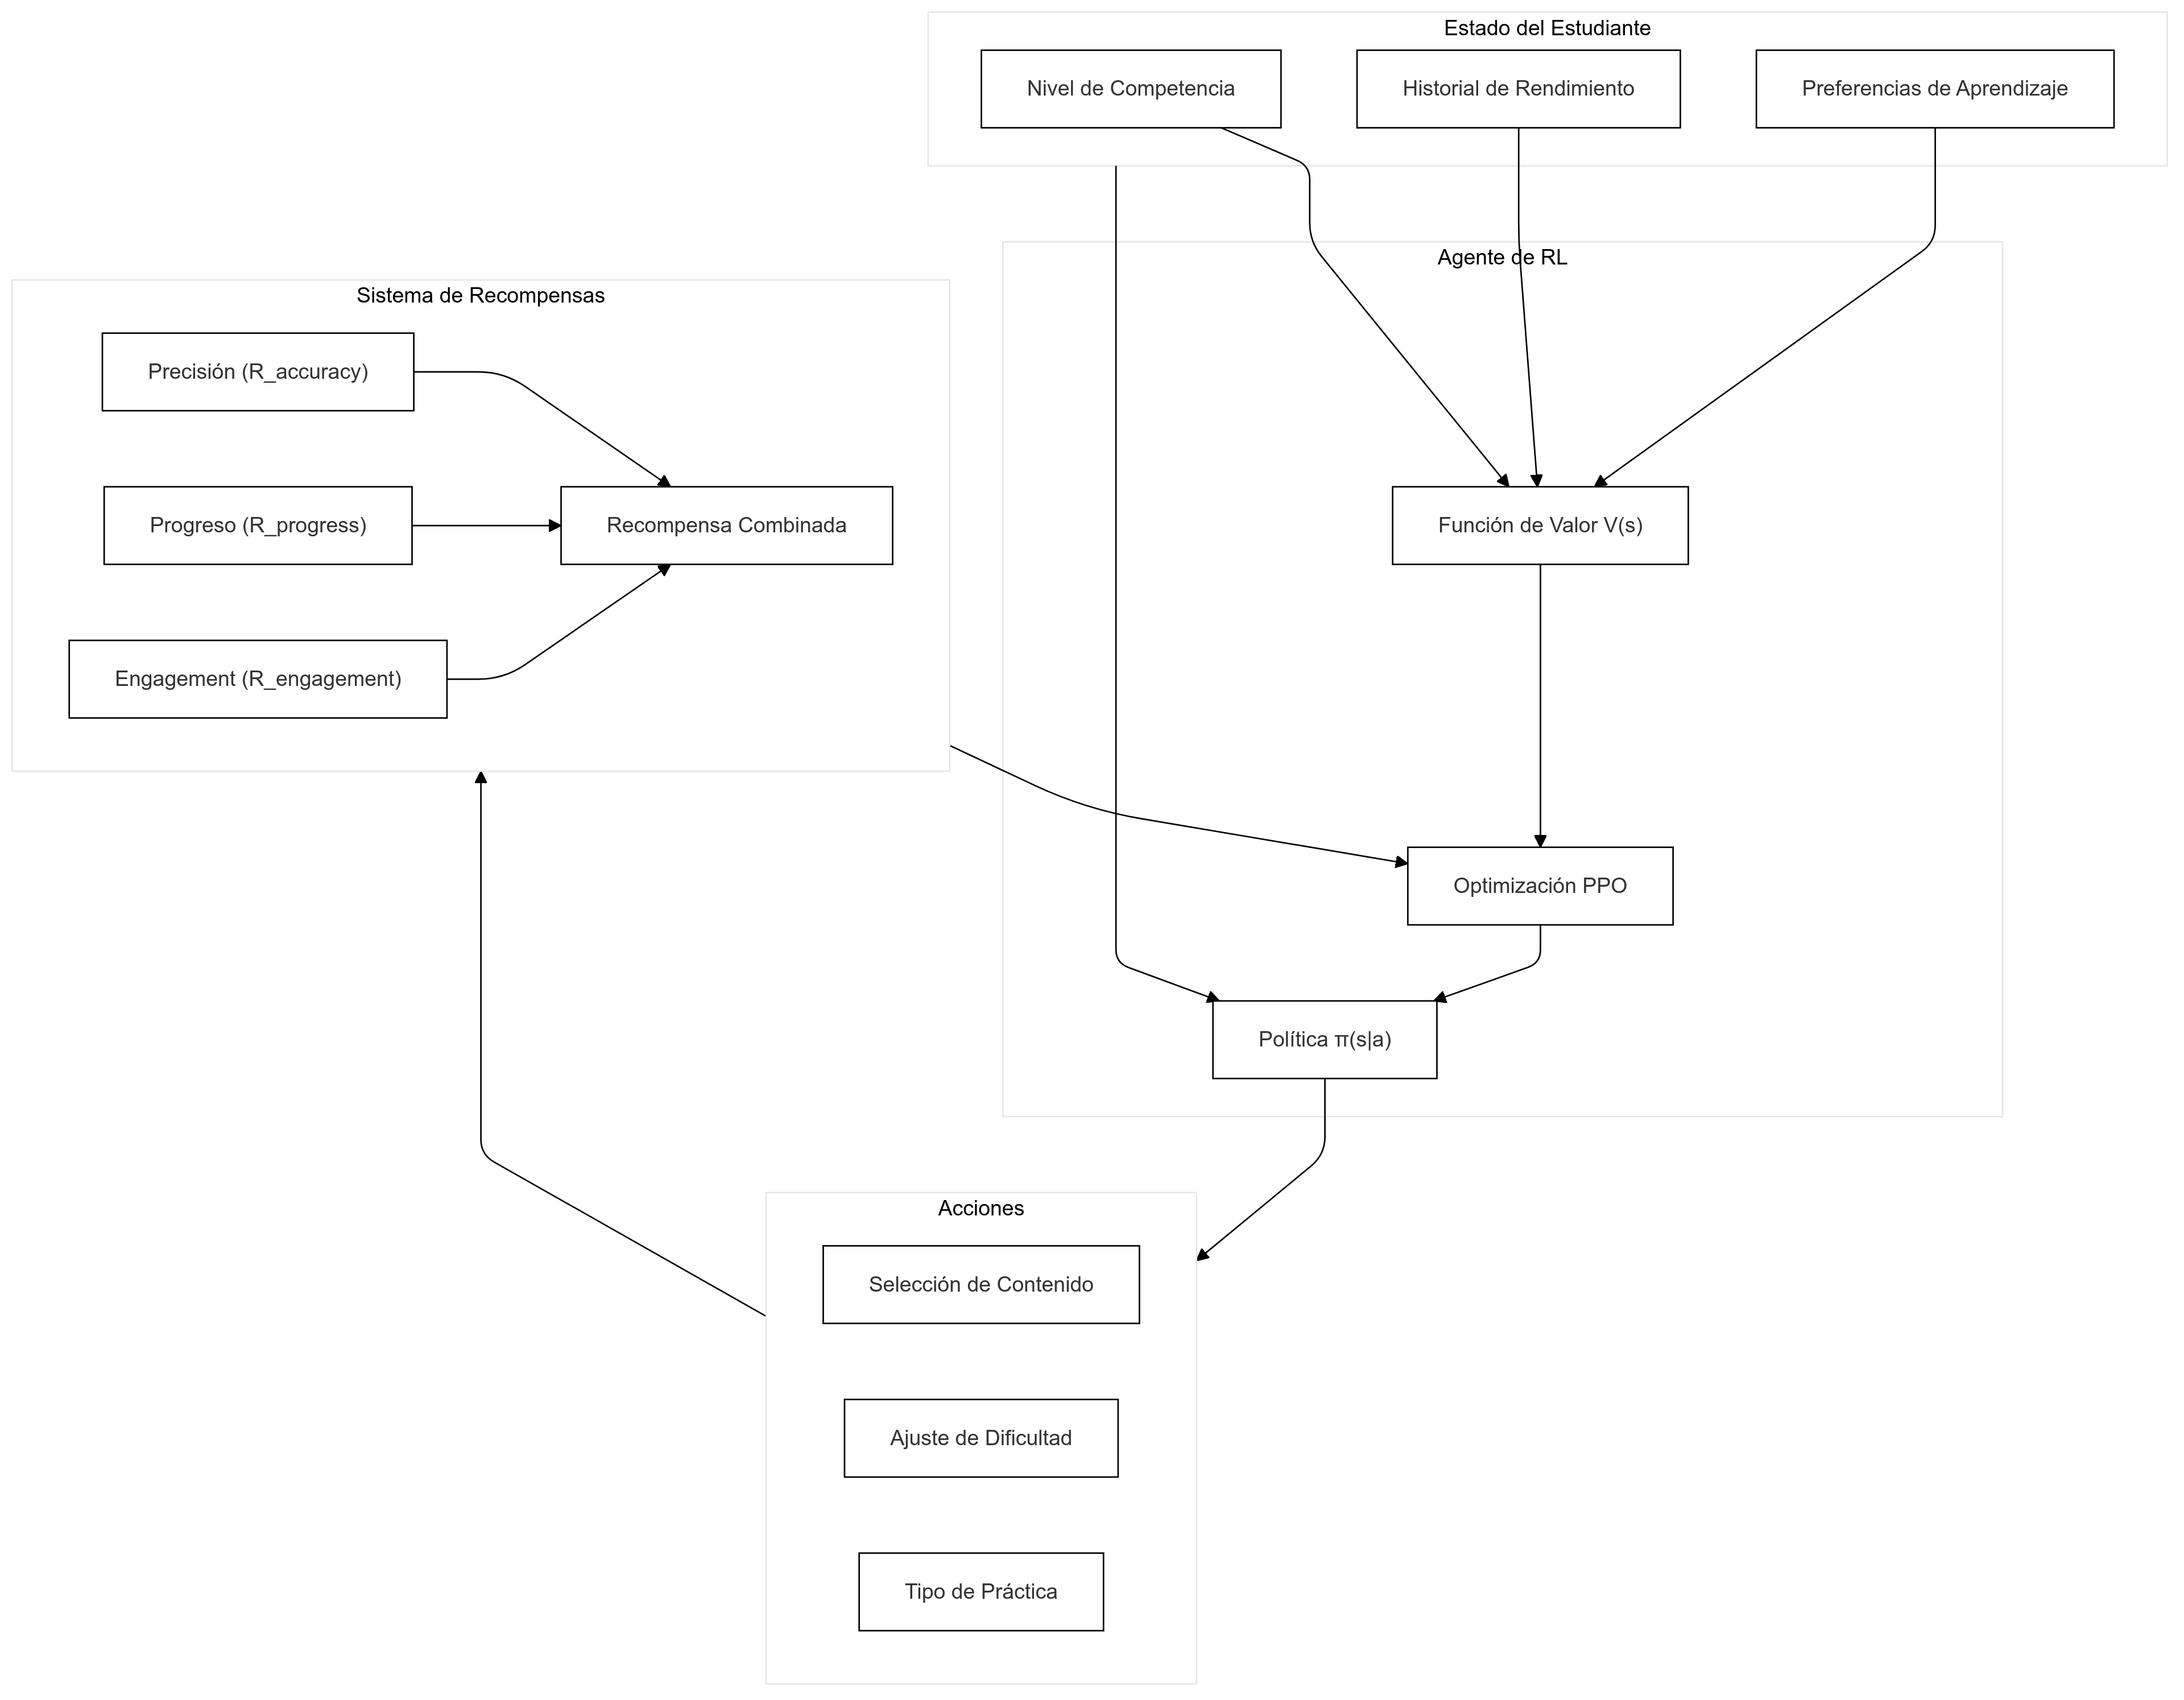
\includegraphics[width=0.8\textwidth]{figuras/rl-flow.png}
\end{figure}

\subsection{Algoritmo de Personalización}
\label{algoritmo-personalizacion}

El sistema implementa un algoritmo de \gls{rl} basado en \gls{ppo} \cite{schulman2017proximal} para optimizar las rutas de aprendizaje. El objetivo es maximizar el aprendizaje a largo plazo mientras se mantiene un nivel apropiado de desafío y engagement.

\subsubsection{Formulación del Problema}

El problema se formula como un \gls{mdp} donde:

\begin{itemize}
	\item \textbf{Estado ($s_t$):} Vector que representa el estado actual del estudiante:
	      \begin{equation}
		      s_t = [c_1, ..., c_n, h_1, ..., h_m, p_1, ..., p_k]
	      \end{equation}
	      donde $c_i$ son los niveles de competencia en diferentes habilidades, $h_i$ es el historial de rendimiento, y $p_i$ son las preferencias de aprendizaje.

	\item \textbf{Acciones ($a_t$):} Vector de decisiones pedagógicas:
	      \begin{equation}
		      a_t = [d, t, c]
	      \end{equation}
	      donde $d$ es el nivel de dificultad, $t$ es el tipo de ejercicio, y $c$ es el contenido específico.

	\item \textbf{Política ($\pi_\theta$):} La política que mapea estados a acciones:
	      \begin{equation}
		      \pi_\theta(a_t|s_t) = P(a_t|s_t; \theta)
	      \end{equation}
\end{itemize}

\subsubsection{Algoritmo PPO}

El algoritmo PPO optimiza la política mediante la siguiente función objetivo:

\begin{equation}
	\label{eq:ppo-objective}
	L^{CLIP}(\theta) = \mathbb{E}_t[\min(r_t(\theta)A_t, \text{clip}(r_t(\theta), 1-\epsilon, 1+\epsilon)A_t)]
\end{equation}

donde:
\begin{itemize}
	\item $r_t(\theta) = \frac{\pi_\theta(a_t|s_t)}{\pi_{\theta_{old}}(a_t|s_t)}$ es el ratio de probabilidades
	\item $A_t$ es la estimación de ventaja
	\item $\epsilon$ es el parámetro de recorte (típicamente 0.2)
\end{itemize}

La actualización de la política se realiza mediante descenso de gradiente:

\begin{equation}
	\theta_{new} = \theta + \alpha \nabla_\theta L^{CLIP}(\theta)
\end{equation}

\subsection{Sistema de Recompensas}
\label{sistema-recompensas}

Se implementa un sistema de recompensas multiobjetivo que considera tres componentes principales:

\begin{equation}
	\label{eq:reward}
	R = w_1R_{accuracy} + w_2R_{progress} + w_3R_{engagement}
\end{equation}

\subsubsection{Componentes de Recompensa}

\begin{itemize}
	\item \textbf{Precisión ($R_{accuracy}$):} Evalúa la corrección de las respuestas:
	      \begin{equation}
		      R_{accuracy} = \frac{\text{respuestas\_correctas}}{\text{total\_respuestas}} \cdot \gamma
	      \end{equation}
	      donde $\gamma$ es un factor de dificultad que aumenta la recompensa para ejercicios más desafiantes.

	\item \textbf{Progreso ($R_{progress}$):} Mide el avance en el dominio de habilidades:
	      \begin{equation}
		      R_{progress} = \sum_{i=1}^n \Delta c_i \cdot \beta_i
	      \end{equation}
	      donde $\Delta c_i$ es el cambio en el nivel de competencia de la habilidad $i$, y $\beta_i$ es su peso relativo.

	\item \textbf{Engagement ($R_{engagement}$):} Evalúa la participación activa:
	      \begin{equation}
		      R_{engagement} = \alpha_t t_{session} + \alpha_c c_{completion} + \alpha_i i_{interaction}
	      \end{equation}
	      donde $t_{session}$ es la duración de la sesión, $c_{completion}$ es la tasa de finalización, y $i_{interaction}$ es la frecuencia de interacción.
\end{itemize}

\subsubsection{Adaptación de Pesos}

Los pesos $w_i$ se ajustan dinámicamente según el perfil del estudiante mediante un algoritmo de adaptación:

\begin{equation}
	w_i^{new} = w_i + \eta(\bar{R}_i - R_{target}) + \lambda\Delta w_i
\end{equation}

donde:
\begin{itemize}
	\item $\eta$ es la tasa de adaptación
	\item $\bar{R}_i$ es la recompensa promedio reciente para el componente $i$
	\item $R_{target}$ es el valor objetivo
	\item $\lambda\Delta w_i$ es un término de momentum para estabilizar los cambios
\end{itemize}

\section{Metodología de Evaluación}
\label{metodologia-evaluacion}

La evaluación del sistema se realiza en dos dimensiones principales: rendimiento técnico y experiencia de usuario. Este enfoque permite valorar tanto la eficiencia técnica del sistema como su utilidad práctica para los usuarios.

\subsection{Evaluación de Rendimiento}
\label{evaluacion-rendimiento}

La evaluación técnica del sistema se centra en dos aspectos principales:

\subsubsection{Métricas del Sistema}

\begin{itemize}
	\item \textbf{Latencia de Respuesta:} Se mide el tiempo de respuesta del sistema en diferentes puntos:
	      \begin{itemize}
		      \item Tiempo de procesamiento de solicitudes API
		      \item Latencia en la generación de respuestas
		      \item Tiempo de renderizado en el cliente
	      \end{itemize}

	\item \textbf{Uso de Recursos:}
	      \begin{itemize}
		      \item Consumo de memoria en el cliente
		      \item Utilización de CPU/GPU
	      \end{itemize}
\end{itemize}

\subsubsection{Rendimiento del Procesamiento de Voz}

\begin{itemize}
	\item \textbf{Precisión en Reconocimiento de Voz:}
	      \begin{itemize}
		      \item Tasa de error en la transcripción
		      \item Precisión en diferentes entornos acústicos
		      \item Tiempo de procesamiento
	      \end{itemize}

	\item \textbf{Calidad de Síntesis de Voz:}
	      \begin{itemize}
		      \item Naturalidad de la voz generada
		      \item Consistencia en la pronunciación
		      \item Velocidad de generación
	      \end{itemize}
\end{itemize}

\subsection{Evaluación de Usuario}
\label{evaluacion-usuario}

La evaluación de la experiencia de usuario se realiza mediante un proceso continuo que combina análisis cuantitativo y cualitativo.

\subsubsection{Recopilación de Retroalimentación}

\begin{itemize}
	\item \textbf{Encuestas de Usuario:}
	      \begin{itemize}
		      \item Evaluación de la facilidad de uso
		      \item Satisfacción con las funcionalidades
		      \item Percepción de la utilidad del sistema
	      \end{itemize}

	\item \textbf{Datos Cualitativos:}
	      \begin{itemize}
		      \item Comentarios y sugerencias de usuarios
		      \item Reportes de problemas
		      \item Sugerencias de mejora
	      \end{itemize}
\end{itemize}

\subsubsection{Análisis de Patrones de Uso}

\begin{itemize}
	\item \textbf{Métricas de Uso:}
	      \begin{itemize}
		      \item Duración promedio de las sesiones
		      \item Frecuencia de uso
		      \item Patrones de interacción
	      \end{itemize}

	\item \textbf{Análisis de Comportamiento:}
	      \begin{itemize}
		      \item Funcionalidades más utilizadas
		      \item Puntos de abandono
		      \item Patrones de navegación
	      \end{itemize}
\end{itemize}

\subsection{Análisis de Resultados}

Los resultados de estas evaluaciones se utilizarán para:

\begin{itemize}
	\item Identificar y corregir problemas técnicos
	\item Mejorar la experiencia de usuario
	\item Optimizar el rendimiento del sistema
	\item Guiar el desarrollo de futuras funcionalidades
\end{itemize}